\subsubsection{Hipótesis}
Para este filtro en particular no teniamos una idea predefinida de con que resultados nos ibamos a encontrar al realizar la experimentacion.
Al ser este un filtro muy sencillo sin necesidad de realizar operaciones matematicas en las cuales poder operar con muchos pixeles en simultaneo, la hipotesis era que la diferencia iba a estar dada por la forma de acceder a memoria pero sin esperar significativas diferencias entre una version y otra.

Elegimos tambien agregar 2 versiones extra de asm: una para medir el acceso mas simple pixel a pixel, y otra utilizando operaciones de repeticions para copiar strings, que para este caso tenia sentido aprovechar.

\subsubsection{Resultados obtenidos}

De estos resultados pudimos sacar algunas concluciones, por un lado la version de C funciono marginamlente mejor que la version asm byte a byte, por lo cual suponemos que, por lo menos en funciones en la cuales la cantidad de instrucciones dentro del ciclo es minima, no hay mucho lugar a optimizaciones posibles y el resultado es un poco mejor debido a algun mejor manejo de las variables utilizadas para iterar.

Por otro lado la version que mejor funciono fue la que utiliza la instruccion rep del microprocesador, obteniendo una ganancia del 34\% respecto a la version optimizada de C.
Incluso funciono mejor que la version simd que procesa de a 16 bytes juntos, pero que requiere mas cantidad de instrucciones para realizarlo.

De todas formas la version que utiliza simd funciono 12\% mas rapida que la version  de C con o3.


\begin{table}[!htbp]
	\centering
	\footnotesize
	\begin{tabular}{| c | c | c | c | c |}
		\hline
Pixels &asm (rep movsb)& asm (simd) & c (o3) & asm (byte a byte)\\ \hline
16x16 & 519 & 492 & 608& 821 \\ \hline
32x32  &1319  & 1594 & 2385& 2859\\ \hline
64x64  & 4430 & 5811 & 9398& 10880 \\ \hline
128x128 & 17508 & 22199 & 40104& 42483 \\ \hline
256x256  & 74415  & 100670 & 158598& 173322\\ \hline
512x512   & 272945 & 406759 & 630169& 685997 \\ \hline
1024x1024 & 2374453 & 2142237 & 4106284& 3088009 \\ \hline
2048x2048  & 10541158  & 14051375 & 15710302& 15923283\\ \hline
4096x4096 & 42235970 & 56320833 & 64179899& 65792957 \\ \hline
8192x8192 & 168890652 & 228391061 & 259152207& 266746729 \\ \hline
Tiempo en X& 1x & 1.35x & 1.53x & 1.57x  \\ \hline
Ganancia vs C & 34.83\% & 11.87\%	& 100.00\% & -2.93\% \\ \hline

 
	\end{tabular}
\end{table}


Es interesante ver que en la version con rep, como evoluciona la cantidad de clocks utilizados para procesar una imagen con la misma cantidad de pixels, pero difere si crece en ancho de si crece en alto.
Debido a que la funcion rep solo se aplica para copiar filas, se ve en la imagen como esta optimizacion mejora su relacion a medida que crece el ancho.

\begin{figure}[!h]
	\centering
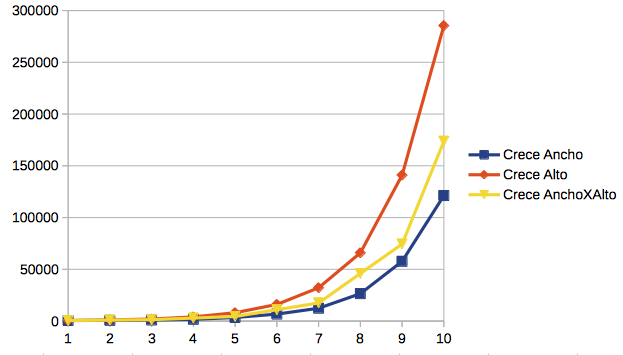
\includegraphics[width=250px]{imgs/crecimientocrop.png}
\end{figure}



